\documentclass[12pt]{scrartcl}
\usepackage[dutch]{babel}
\usepackage{CJK}
\usepackage[CJK, overlap]{ruby}
\usepackage{float}
\usepackage{graphicx}
\usepackage{multirow}

\renewcommand{\rubysep}{-0.2ex}


\begin{document}

%\begin{CJK*}[dnp]{JIS}{min}
\begin{CJK*}{UTF8}{min}
\CJKtilde
%\CJKcaption{JIS}

%
% Title page
%
\title{Aikibudo Terminologie}
\author{Andy Nagels}
\maketitle
\thispagestyle{empty} %should remove the page number
%\pagestyle{empty} %should remove the page number in the whole document
\begin{figure}[H]
\centering
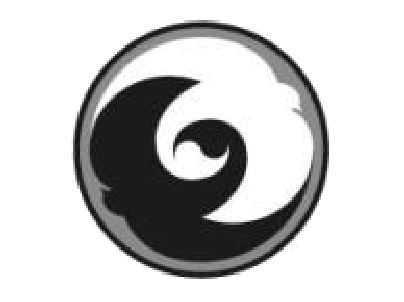
\includegraphics[width=2.5cm]{img/schild_aikibudo.eps}
\end{figure}

\begin{center}
合気武道
\end{center}

\begin{figure}[H]
\centering
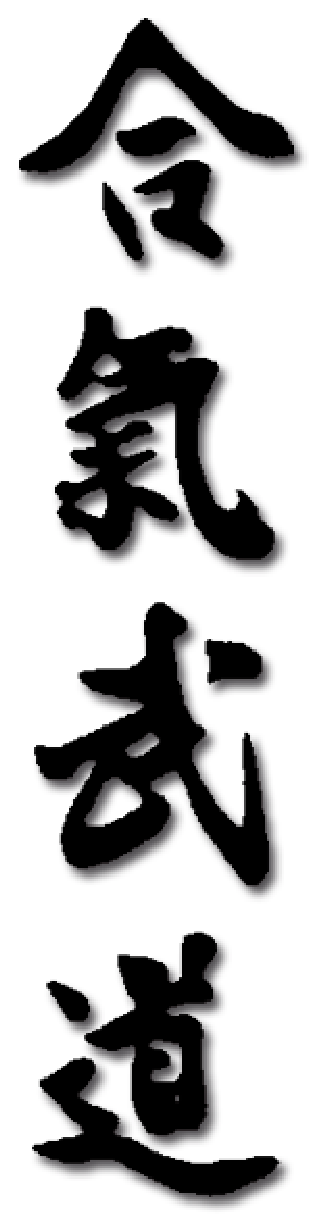
\includegraphics[width=1.0cm]{img/aikibudo-kanji.eps}
\end{figure}

%
% Table of contents
%
\newpage
\setcounter{page}{1}
\pagenumbering{Roman}
\tableofcontents

%
% Main content
%
\newpage
\setcounter{page}{1}
\pagenumbering{arabic}

% standard it's wadalab mincho, which gives the best results
\CJKfamily{goth}

\section{Inleiding}
\noindent Dit document bevat termen die gebruikt worden in aikibudo.

\section{De Japanse taal}
\noindent Alvorens we de berippen bekijken, dient een korte uitleg gegeven te worden over de Japanse taal.\\

\noindent Japans is opgebouwd uit 3 grote onderdelen: \textit{hiragana, katakana} en \textit{kanji}.\\

\noindent Hiragana en katakana zijn allebei een \textit{phonetisch} alfabet. Dat wil zeggen dat het symbolen voorstelt, die een klank uitbeelden.
Japans heeft dus geen aparte letters, zoals de meeste Westerse alfabetten.\\

\noindent \textbf{Hiragana} wordt gebruikt om zinnen te vormen en grammatica toe te passen op de Japanse taal. Het toont hoe Japans wordt uitgesproken.\\

\noindent \textbf{Katakana} bevat dezelfde klanken en enkele extra klanken. Het is ontstaan om de verschillende buitenlandse termen te kunnen uitspreken. Zo worden bvb. namen van niet Japanners in katakana geschreven.\\

\noindent \textbf{Kanji} zijn de meer complexe Japanse symbolen, die woorden en begrippen voorstellen. Ook Japanse namen en plaatsnamen worden meestal met kanji geschreven. Om te weten hoe deze symbolen worden uitgesproken, wordt gebruik gemaakt van hiragana, omdat hiragana een phonetisch alfabet is dat klanken in beeld brengt.\\

\noindent \textbf{Romaji} is een westerse schrijfwijze van Japanse klanken. Het wordt in Japan ook gebruikt om op een computer te typen.
Het is deze schrijfwijze, die het mogelijk maakt voor mensen die geen Japans kennen, om Japanse termen correct uit te spreken.

\noindent In de tabel hieronder, kan je een overzicht vinden van de verschillende alfabetten, ter verduidelijking van bovenstaande uitleg.\\

\begin{table}[H]
\begin{center}
\begin{tabular}{c|c|c|c}
Nederlands alfabet & Hiragana & Katakana & Romaji\\
\hline
a &  あ & ア & a\\
k & bestaat niet & bestaat niet & bestaat niet\\
bestaat niet & か & カ & ka
\end{tabular}
\end{center}
\caption{Een kleine vergelijking ter verduidelijking}
\label{vergelijking_alfabetten}
\end{table}

\noindent De begrippen in dit document, zijn op volgende manier weergegeven:\\

\textit{Nederlandse omschrijving} $|$ \textit{Japanse term (hiragana uitspraak)} $|$ \textit{romaji uitspraak}\\

\noindent De technieken zijn echter te lang om op die manier weer te geven. Zij staan dus onder elkaar:\\

\begin{center}
\textit{Nederlandse term}\\
\textit{Japanse term (hiragana uitspraak)}\\
\textit{Romaji uitspraak}
\end{center}

\section{Uitspraak}
\noindent Een aantal letters worden iets anders uitgesproken in de romaji uitspraak, t.o.v. het Nederlands.
Het is interessant om dit even te lezen, om zo geen verkeerde uitspraak te leren voor de techniek.\\

\noindent j: $|zj|$ zoals in strand\textbf{j}anet, \textbf{J}efke, ... (en NIET zoals in \textbf{J}ommeke)\\
ch: $|tsj|$ zoals in \textbf{tsj}oeke \textbf{tsj}oeke tuut tuut\\
sh: $|sj|$ zoals in \textbf{ch}oco, \textbf{sh}ampoo, ...\\
u: korte $|oe|$ zoals in nen t\textbf{oe}k \textbf{oe}p aa bakkes, vake en m\textbf{oe}ke, ...\\
\={o} of ou: lange $|o|$ zoals in b\textbf{oo}t

\section{Algemene terminologie}
\subsection{Algemeen}
\begin{table}[H]
\begin{center}
\begin{tabular}{c|c|c}
basis/oorsprong/standaard & 基本 (きほん) & kihon \\
\hline
de kunst van het veilig vallen & 受身 (うけみ) & ukemi \\
\hline
actieve partner & 取り(どり) & dori\\
\hline
controle & 押さえ (おさえ) & osae\\
\hline
techniek & 技 (わざ) & waza\\
\hline
houding & 構え (かまえ) & kamae 
\end{tabular}
\end{center}
\end{table}

\subsection{Richtingen en gebieden}
\begin{table}[H]
\begin{center}
\begin{tabular}{c|c|c}
rechts & 右 (みぎ) & migi \\
\hline
links & 左 (ひだり) & hidari\\
\hline
achterwaarts & 後ろ(うしろ) & ushiro\\
\hline
voorwaarts & 前 (まえ) & mae\\
\hline
bovenste graad & 上段 (じょうだん) & j\={o}dan\\
\hline
midden & 中段 (ちゅうだん) & chuudan\\
\hline
grond & 土(ど) & do
\end{tabular}
\end{center}
\end{table}

\subsection{Acties}
\begin{table}[H]
\begin{center}
\begin{tabular}{c|c|c}
worp & 投げ (なげ) & nage\\
\hline
kopstoot & 頭突き (ずつき) & zutsuki\\
\hline
trap & 蹴り (けり) & keri\\
\hline
wurging & 絞殺 (こうさつ) & k\={o}satsu\\
\hline
omkering/terug sturen & 返し (がえし) & gaeshi\\
\hline
zijwaartse trap & 横蹴り (よこけり) & yoko keri\\
\hline
stoot & 突き (つき) & tsuki
\end{tabular}
\end{center}
\end{table}

\subsection{Lichaamsdelen}
\begin{table}[H]
\begin{center}
\begin{tabular}{c|c|c}
lichaam & 体 (たい) & tai \\
\hline
hand & 手(て) & te \\
\hline
elleboog/elleboogstoot & 肘 (ひじ) & hiji\\
\hline
knie & 膝 (ひざ) & hiza\\
\hline
pols & 手首 (てくび) & tekubi\\
\hline
onderarm & 小手 (こて) & kote\\
\hline
schouder & 肩 (かた) & kata
\end{tabular}
\end{center}
\end{table}

\subsection{Andere begrippen}
\begin{table}[H]
\begin{center}
\begin{tabular}{c|c|c}
schroef/veer van horloge & 捻子 (ねじ) & neji\\
\hline
tabel & 表 (おもて) & omote
\end{tabular}
\end{center}
\end{table}

\subsection{Leerstof}
\begin{table}[H]
\begin{center}
\begin{tabular}{c|c|c}
verwijdering van het lichaam & 体捌き (たいさばき) & tai sabaki\\
\hline
valtechnieken & 受身技 (うけみわざ) & ukemi waza\\
\hline
stoottechnieken & 突き技 (つきわざ) & tsuki waza\\
\hline
traptechnieken & 蹴り技 (けりわざ) & keri waza\\
\hline
? & ? (ほじょうんど) & hojo undo\\
\hline
vrij gevecht & 乱取り (らんどり) & randori
\end{tabular}
\end{center}
\end{table}

\newpage
\section{Kyu technieken}
\subsection{6de kyu (SHOKU)}
\begin{table}[H]
\begin{center}
\begin{tabular}{c|c}
\textbf{verwijdering van het lichaam} & ?\\
\textbf{体捌き (たいさばき)} & ? (いりみ)\\
\textbf{tai sabaki} & irimi\\
\cline{2-2}
& ?\\
& ? (おいりみ)\\
& o irimi\\
\hline
\textbf{valtechnieken} & achterwaarts\\
\textbf{受身技 (うけみわざ)} & 後ろ (うしろ)\\
\textbf{ukemi waza} & ushiro\\
\hline
\textbf{stoottechnieken} & ?\\
\textbf{突き技 (つきわざ)} & ?\\
\textbf{tsuki waza} & ? \\
\hline
\end{tabular}
\end{center}
\label{kyu_6}
\end{table}

\newpage
\subsection{5de kyu (SHOKU)}

\newpage
\subsection{4de kyu (CHUKYU)}

\newpage
\subsection{3de kyu (CHUKYU)}

\newpage
\subsection{2de kyu (JOKYU)}

\newpage
\subsection{1de kyu (JOKYU)}

\newpage
\section{Dan technieken}
\subsection{1ste dan}
\begin{table}[H]
\begin{center}
\begin{tabular}{c}
?\\
? (ひらき)\\
hiraki\\
\hline
weegschaal worp\\
天秤投げ (てんびんあげ)\\
tenbin nage\\
\hline
veer/schroef van horloge onderarm omkering\\
螺子小手返し (ねじこてがえし)\\
neji kote gaeshi\\
\hline
?\\
螺子小手返し (ねじこてがえし)\\
\end{tabular}
\end{center}
\label{dan_1}
\end{table}

\newpage
\subsection{2de dan}

\newpage
\subsection{3de dan}

\newpage
\section{表技 Omote waza}
\subsection{基本投げ技 Kihon nage waza (7 technieken)}

\subsection{基本押さえ技 Kihon osae waza (6 technieken)}

\subsection{?技 投げ技 Oyo waza nage waza (間 - ??)}

\subsection{?技 押さえ技 Oyo waza osae waza (間 - ??)}

\newpage
\section{Tenshin Sh\={o}den Katori Shinto Ryu}
\subsection{Algemeen}
\begin{table}[H]
\begin{center}
\begin{tabular}{c}
naieve authentieke biografie van Katori God\\
天真(てんしんしょうでんかとりしんとりゅ)\\
tenshin sh\={o}den katori shinto ryu
\end{tabular}
\end{center}
\label{katori}
\end{table}


\subsection{6de kyu}
\begin{table}[H]
\begin{center}
\begin{tabular}{c}
bovenste/hoge houding\\
上段の構え(じょうだんのかまえ)\\
j\={o}dan no kamae\\
\hline
houding van de blik (katana laten zakken om het zicht vrij te maken)\\
正眼の構え(せいがんのかまえ)\\
seigan no kamae\\
\hline
boog onder een hoek\\
弧がすみ(こがすみ)\\
ko gasumi\\
\hline
hand naar achteren onder een hoek\\
手裏がすみ(てるあがすみ)\\
te ura gasumi
\end{tabular}
\end{center}
\label{kyu_1_katori}
\end{table}

\end{CJK*}
\end{document}
